\section{1174027 - Harun Ar - Rasyid}
\subsection{Teori}
\begin{enumerate}
	\item Jelaskan apa itu klasifikasi teks, sertakan gambar ilustrasi buatan sendiri.
	\hfill\break
	Klasifikasi teks adalah proses pemberian tag atau kategori ke teks sesuai dengan isinya. Teks dapat menjadi sumber informasi yang sangat kaya, tetapi mengekstraksi wawasan darinya bisa sulit dan memakan waktu karena sifatnya yang tidak terstruktur. berikut contoh gambar .
	\begin{figure}[H]
		\centering
		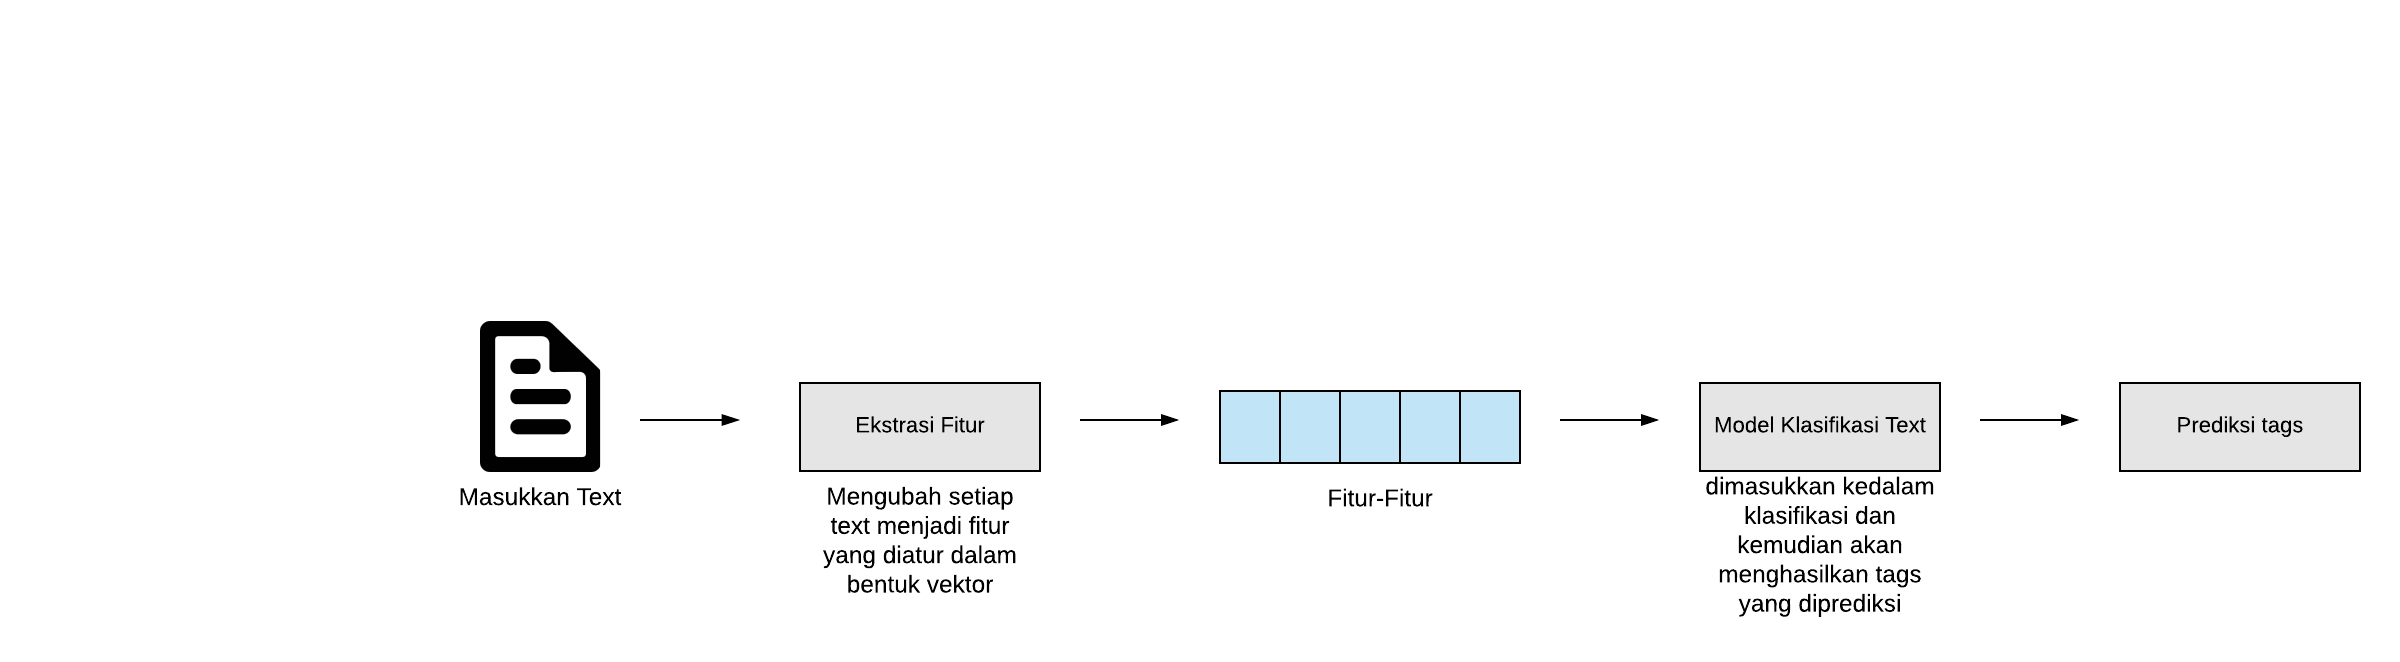
\includegraphics[width=4cm]{figures/1174027/4/1.png}
		\caption{Ilustrasi Klasifikasi.}
	\end{figure}
	\item Jelaskan mengapa klasifikasi bunga tidak bisa menggunakan machine learning, sertakan ilustrasi sendiri.
	\hfill\break
    Untuk klasifikasi bunga tidak dapat menggunakan machine learning dikarenakan memiliki masalah input yang sama namun keluarannya (output) yang berbeda, biasanya output atau error ini disebut dengan istilah ’noise’. Noise sendiri merupakan output yang disimpan / ditangkap maupun direkam bukan seperti seharusnya ( keluaran yang diiginkan ). Apabila diberikan contoh, maka contohnya yaitu kita berasumsi secara implisit bahwa klarifikasi bunga yang kita lakukan sudah tepat dan kita melakukannya seperti seorang ahli tanaman. Namun pada hasilnya masih saja terjadi kesalahan. Selain itu, selalu ada peluang untuk memperkenalkan kesalahan saat merekam ataupun menyimpan data, maka harus dilakukan penelitian yang lebih rinci sehingga tidak menimbulkan ’noise’ itu sendiri.
	\begin{figure}[H]
		\centering
		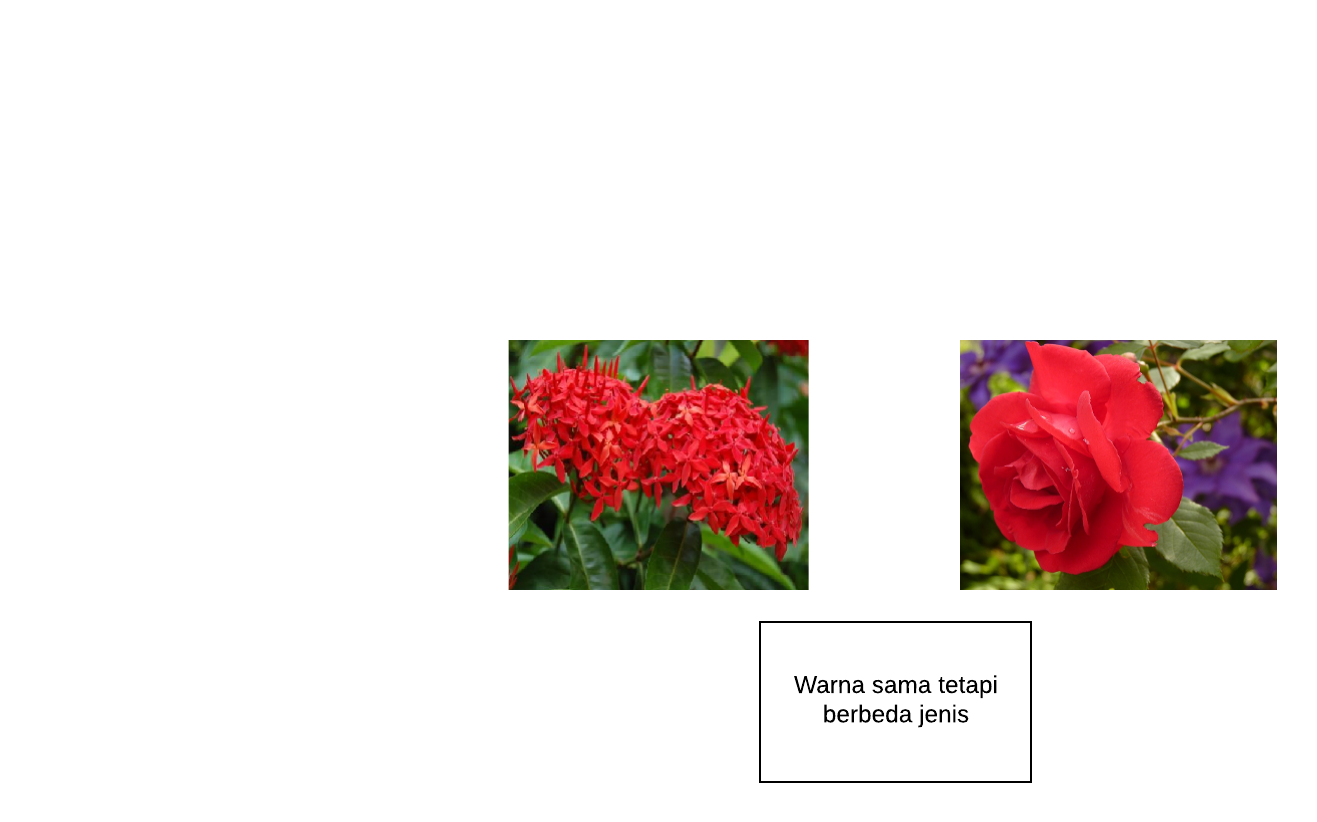
\includegraphics[width=4cm]{figures/1174027/4/2.png}
		\caption{Ilustrasi klasifikasi bunga.}
	\end{figure}
	\item Jelaskan bagaimana teknik pembelajaran mesin pada teks pada kata-kata yang digunakan di youtube,jelaskan arti per atribut data csv dan sertakan ilustrasi buatan sendiri.
	\hfill\break
	Kita ambil sebuah kasus yang semua orang telah ketahui dan juga pahami. Kasus tersebut yaitu perekomendasian video dari pencarian menggunakan ”text / kata” di Youtube. Pada saat menggunakan Youtube terdapat Machine Learning yang bekerja dan memproses perintah ataupun aktivitas tersebut, dimana akan memfilter secara otomatis video yang disesuaikan dengan ”keyword” yang kita masukkan sehingga memberikan keluaran video dengan keyword yang benar. Adapula fitur yang di dapatkan ketika sedang menonton Youtube. Tampilan sebelah kanan terdapat pilihan ’Next’ atapun ’Suggestion’ yang menampilkan beberapa video serupa sesuai dengan yang dicari atau sedang ditonton. Ketika mengklik salah satu video dari baris tersebut, maka Youtube akan mengingat dan menggunakan kata yang tertera sebagai referensi kembali sehingga akan memberikan kemudahan pada pencarian yang lainnya, Dan disitulah mesin belajar sendiri dan menyimpan data secara berkala sehingga berkembang.
    \begin{figure}[H]
		\centering
		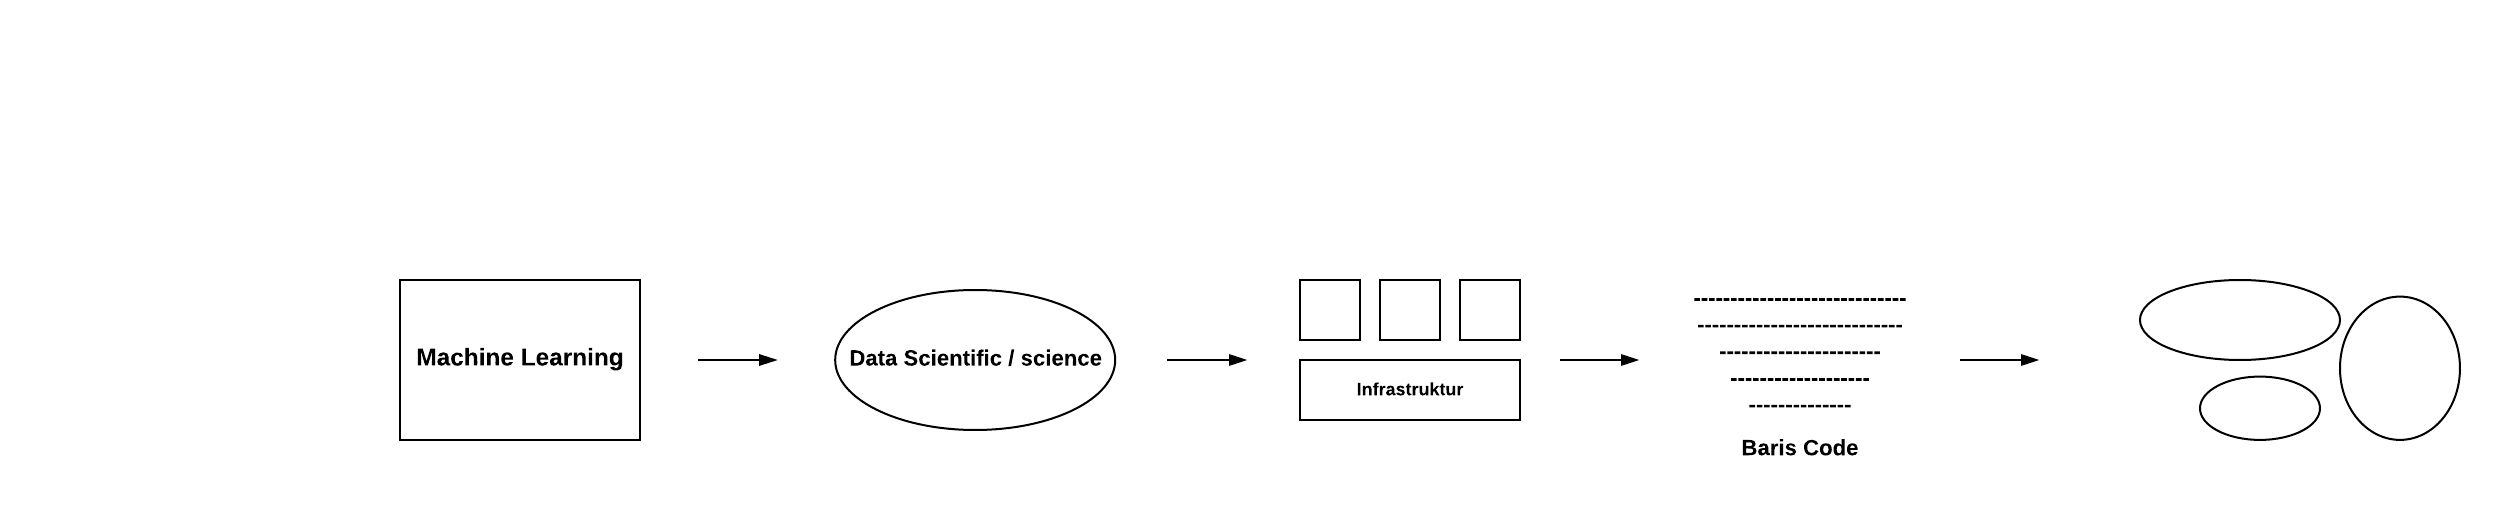
\includegraphics[width=4cm]{figures/1174027/4/3.png}
		\caption{Ilustrasi Teknik Pembelajaran Mesin.}
	\end{figure}

	\item Jelaskan apa yang dimaksud vektorisasi data.
	\hfill\break
	Pembagian dan pemecahan data, kemudian dilakukan perhitungan. Vektorisasi juga dapat dimaksudkan dengan setiap data yang mungkin dipetakan ke integer tertentu. jika kita memiliki array yang cukup besar maka setiap kata / data cocok dengan slot unik dalam array (nilai pada indeks adalah nomor satu kali kata itu muncul).
    \hfill\break
	Array angka floating point ( Mewakili data ) :
	\begin{itemize}
		\item teks
    	\item audio
    	\item gambar
	\end{itemize}

	Contoh : -[1.0, 0.0, 1.0, 0.5]

	\item Jelaskan apa itu bag of words dengan kata-kata yang sederhana dan ilustrasi sendiri.
	\hfill\break
	bag-of-words adalah representasi penyederhanaan yang digunakan dalam pemrosesan bahasa alami dan pengambilan informasi. Model bag-of-words sederhana untuk dipahami dan diterapkan dan telah melihat kesuksesan besar dalam masalah seperti pemodelan bahasa dan klasifikasi dokumen.Pada model ini, tiap kalimat dalam dokumen digambarkan sebagai token, mengabaikan tata bahasa dan bahkan urutan kata namun menghitung frekuensi kejadian atau kemunculan kata dari dokumen.
	\begin{figure}[H]
		\centering
		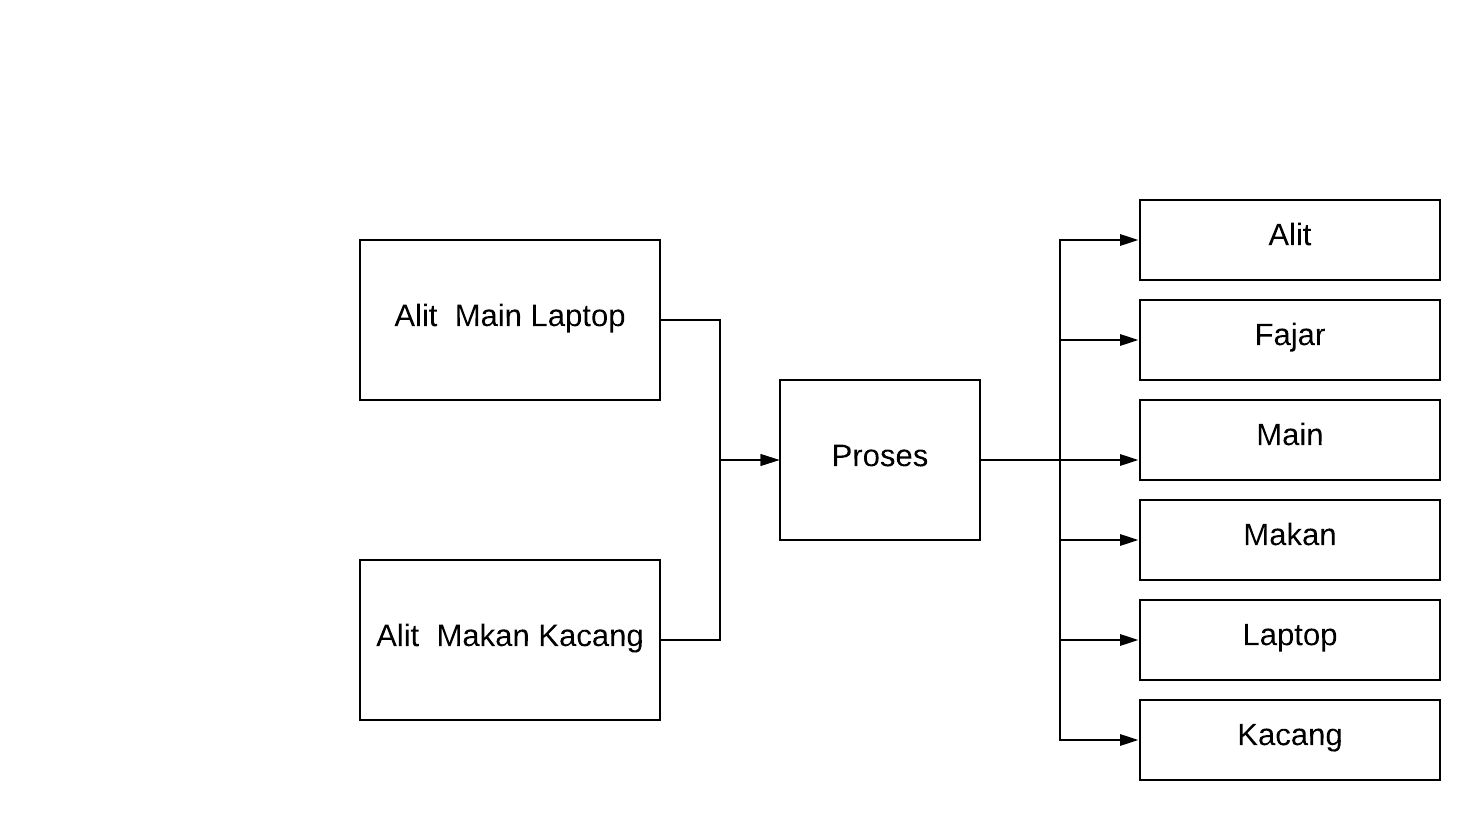
\includegraphics[width=4cm]{figures/1174027/4/4.png}
		\caption{Ilustrasi Bag of words.}
	\end{figure}

	\item Jelaskan apa itu TF-IDF, ilustrasikan dengan gambar sendiri
	\hfill\break
	TF-IDF memberi kita frekuensi kata dalam setiap dokumen dalam korpus atau mengganti data jadi number. Ini adalah rasio berapa kali kata itu muncul dalam dokumen dibandingkan dengan jumlah total kata dalam dokumen itu. Itu meningkat seiring jumlah kemunculan kata itu di dalam dokumen meningkat. Setiap dokumen memiliki tf sendiri.
	\begin{figure}[H]
		\centering
		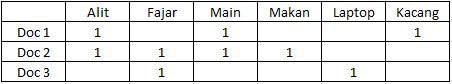
\includegraphics[width=4cm]{figures/1174027/4/5.png}
		\caption{Ilustrasi TF IDF.}
	\end{figure}
\end{enumerate}
\subsection{Praktek}
\begin{enumerate}
	\item import data pandas dan 500 baris data dummy kemudian di jelaskan tiap barisnya.
	\hfill\break
	\lstinputlisting[firstline=8, lastline=18]{src/1174027/4/1174027.py}

	\item Dari dataframe tersebut dipecah menjadi dua dataframe yaitu 450 row pertama dan 50 row sisanya
	\hfill\break
	\lstinputlisting[firstline=21, lastline=25]{src/1174027/4/1174027.py}

	\item Pratekkan vektorisasi dan klasifikasi dari data (NPM mod 4, jika 0 maka katty perry, 1 LMFAO, 2 Eminem, 3 Shakira) dengan Decission Tree. Tunjukkan keluarannya dari komputer sendiri dan artikan maksud setiap luaran yang didapatkan.
	\hfill\break
	\lstinputlisting[firstline=26, lastline=59]{src/1174027/4/1174027.py}

	\item Cobalah klasifikasikan dari data vektorisasi yang di tentukan di nomor sebelumnya dengan klasifikasi SVM. Tunjukkan keluarannya dari komputer sendiri dan artikan maksud setiap luaran yang didapatkan.
	\hfill\break
	\lstinputlisting[firstline=60, lastline=66]{src/1174027/4/1174027.py}
	
	\item Cobalah klasifikasikan dari data vektorisasi yang di tentukan di nomor sebelumnya dengan klasifikasi Decission Tree. Tunjukkan keluarannya dari komputer sendiri dan artikan maksud setiap luaran yang didapatkan.
    \hfill\break
	\lstinputlisting[firstline=67, lastline=72]{src/1174027/4/1174027.py}
	
	\item Plotlah confusion matrix dari praktek modul ini menggunakan matplotlib.Tunjukkan keluarannya dari komputer sendiri dan artikan maksud setiap luaran yang didapatkan.
    \hfill\break
	\lstinputlisting[firstline=73, lastline=78]{src/1174027/4/1174027.py}
	
	\item Jalankan program cross validaiton pada bagian teori bab ini. Tunjukkan keluarannya dari komputer sendiri dan artikan maksud setiap luaran yang didapatkan.
	\hfill\break
	\lstinputlisting[firstline=79, lastline=99]{src/1174027/4/1174027.py}
	
	\item Buatlah program pengamatan komponen informasi pada bagian teori bab ini. Tunjukkan keluarannya dari komputer sendiri dan artikan maksud setiap luaran yang didapatkan.
	\hfill\break
	\lstinputlisting[firstline=100, lastline=135]{src/1174027/4/1174027.py}
\end{enumerate}
\subsection{Penangan error}
\begin{enumerate}
	\item ScreenShoot Error
	\begin{figure}[H]
		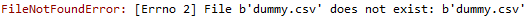
\includegraphics[width=4cm]{figures/1174027/error/4_file_not_found.png}
		\centering
		\caption{FileNotFoundError}
	\end{figure}
	\item Tuliskan Kode Error dan Jenis Error
	\begin{itemize}
		\item FileNotFoundError
	\end{itemize}
	\item Cara Penangan Error
	\begin{itemize}
		\item FileNotFoundError
		\hfill\break
		Error terdapat pada kesalahan baca file csv, yang tidak terbaca. Dikarenakan letak file yang dibaca tidak para direktori yang sama. Seharusnya letakkan file di direktori yang sama. 
	\end{itemize}
\end{enumerate}
\subsection{Bukti Tidak Melakukan Plagiat}
\begin{figure}[H]
	\centering
		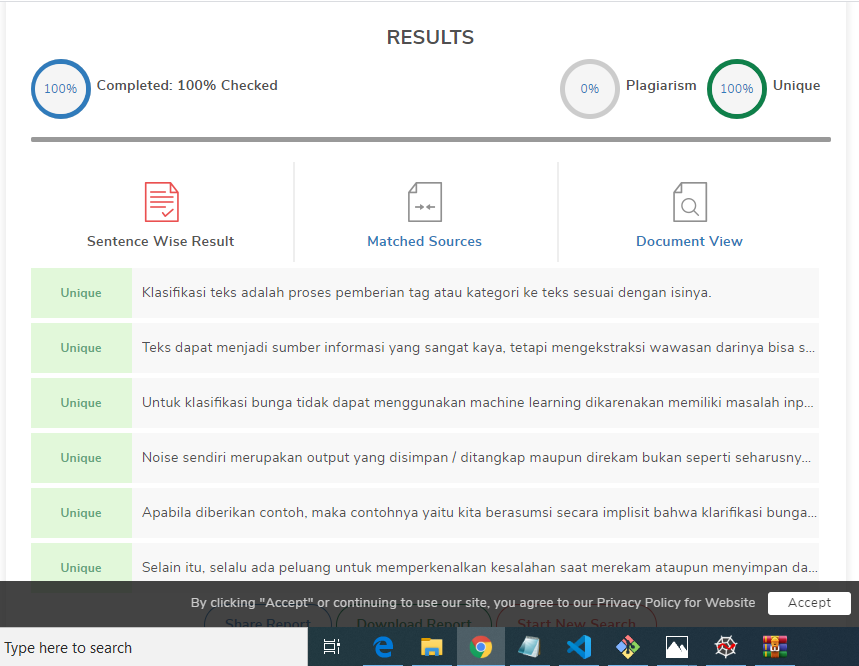
\includegraphics[width=4cm]{figures/1174027/bukti/4.png}
		\caption{Bukti Tidak Melakukan Plagiat Chapter 4}
	\end{figure}